\pagebreak
\thispagestyle{empty}
\movetoevenpage
\begin{figure}
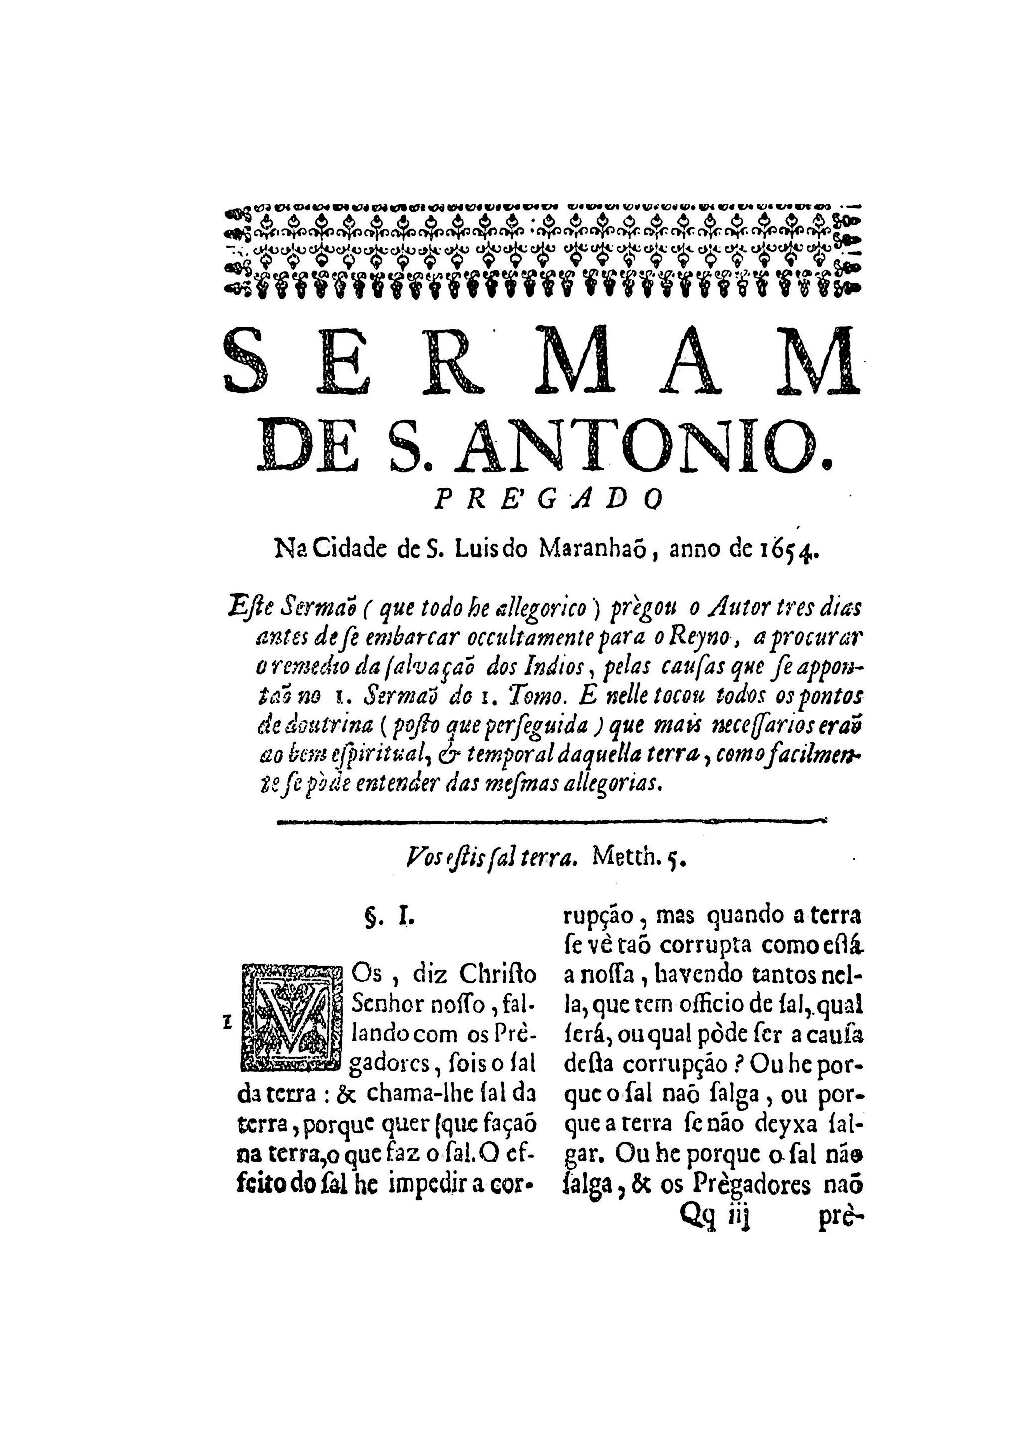
\includegraphics[width=\textwidth]{./imgs/stantonio.pdf}  
\end{figure}

\chapter{Sermão de Santo Antonio}

\begin{quotation}
\noindent{}Pregado na Cidade de S.\,Luís do Maranhão, ano de 1654.
Esse Sermão (que todo é alegórico) pregou o Autor três dias antes de se embarcar
ocultamente para o Reino, a procurar o remédio da salvação dos Índios, pelas
causas que se apontam no \textsc{i} Sermão do \textsc{i} Tomo. E nele
tocou os pontos de doutrinas (posto que perseguida) que mais necessários eram ao bem espiritual, e temporal daquela terra, como facilmente se pode entender das mesmas alegorias.
\end{quotation}

\epigraph{\emph{Vos estis sal terrae}.}{S.\,Mateus, \textsc{v}, l3.}

\section*{i}

\noindent{}Vós, diz Cristo, Senhor nosso, falando com os pregadores, sois o sal da
terra: e chama"-lhes sal da terra, porque quer que façam na terra o que
faz o sal. O efeito do sal é impedir a corrupção; mas quando a terra se
vê tão corrupta como está a nossa, havendo tantos nela que têm ofício de
sal, qual será, ou qual pode ser a causa desta corrupção? Ou é porque o
sal não salga, ou porque a terra se não deixa salgar. Ou é porque o sal
não salga, e os pregadores não pregam a verdadeira doutrina; ou porque a
terra se não deixa salgar e os ouvintes, sendo verdadeira a doutrina que
lhes dão, a não querem receber. Ou é porque o sal não salga, e os
pregadores dizem uma cousa e fazem outra; ou porque a terra se não deixa
salgar, e os ouvintes querem antes imitar o que eles fazem, que fazer o
que dizem. Ou é porque o sal não salga, e os pregadores se pregam a si e
não a Cristo; ou porque a terra se não deixa salgar, e os ouvintes, em
vez de servir a Cristo, servem a seus apetites. Não é tudo isto verdade?
Ainda mal!

Suposto, pois, que ou o sal não salgue ou a terra se não deixe salgar;
que se há e fazer a este sal e que se há e fazer a esta terra? O que se
há e fazer ao sal que não salga, Cristo o disse logo: \emph{Quod si sal
evanuerit, in quo salietur? Ad nihilum valet ultra, nisi ut mittatur
foras et conculcetur ab hominibus}. Se o sal perder a substância e a
virtude, e o pregador faltar à doutrina e ao exemplo, o que se lhe há e
fazer, é lançá"-lo fora como inútil para que seja pisado de todos. Quem
se atrevera a dizer tal cousa, se o mesmo Cristo a não pronunciara?
Assim como não há quem seja mais digno de reverência e de ser posto
sobre a cabeça que o pregador que ensina e faz o que deve, assim é
merecedor de todo o desprezo e de ser metido debaixo dos pés, o que com
a palavra ou com a vida prega o contrário.

Isto é o que se deve fazer ao sal que não salga. E à terra que se não
deixa salgar, que se lhe há de fazer? Este ponto não resolveu Cristo,
Senhor nosso, no Evangelho; mas temos sobre ele a resolução do nosso
grande português Santo Antônio, que hoje celebramos, e a mais galharda e
gloriosa resolução que nenhum santo tomou.
Pregava Santo Antônio em Itália na cidade de Arimino, contra os hereges,
que nela eram muitos; e como erros de entendimento são dificultosos de
arrancar, não só não fazia fruto o santo, mas chegou o povo a se
levantar contra ele e faltou pouco para que lhe não tirassem a vida. Que
faria neste caso o ânimo generoso do grande Antônio? Sacudiria o pó dos
sapatos, como Cristo aconselha em outro lugar? Mas Antônio com os pés
descalços não podia fazer esta protestação; e uns pés a que se não pegou
nada da terra não tinham que sacudir. Que faria logo? Retirar"-se"-ia?
Calar"-se"-ia? Dissimularia? Daria tempo ao tempo? Isso ensinaria
porventura a prudência ou a covardia humana; mas o zelo da glória
divina, que ardia naquele
peito, não se rendeu a semelhantes partidos. Pois que fez? Mudou somente
o púlpito e o auditório, mas não desistiu da doutrina. Deixa as praças,
vai"-se às praias; deixa a terra, vai"-se ao mar, e começa a dizer a altas
vozes: Já que me não querem ouvir os homens, ouçam"-me os peixes. Oh
maravilhas do Altíssimo! Oh poderes do que criou o mar e a terra!
Começam a ferver as ondas, começam a concorrer os peixes, os grandes, os
maiores, os pequenos, e postos todos por sua ordem com as cabeças de
fora da água, Antônio pregava e eles ouviam.

Se a Igreja quer que preguemos de Santo Antônio sobre o Evangelho,
dê"-nos outro. \emph{Vos estis sal terrae}: É muito bom texto para os
outros santos doutores; mas para Santo Antônio vem"-lhe muito curto. Os
outros santos doutores da Igreja foram sal da terra; Santo Antônio foi
sal da terra e foi sal do mar. Este é o assunto que eu tinha para tomar
hoje. Mas há muitos dias que tenho metido no pensamento que, nas festas
dos santos, é melhor pregar como eles, que pregar deles. Quanto mais que
o são da minha doutrina, qualquer que ele seja tem tido nesta terra uma
fortuna tão parecida à de Santo Antônio em Arimino, que é força segui"-la
em tudo. Muitas vezes vos tenho pregado nesta igreja, e noutras, de
manhã e de tarde, de dia e de noite, sempre com doutrina muito clara,
muito sólida, muito verdadeira, e a que mais necessária e importante é a
esta terra para emenda e reforma dos vícios que a corrompem. O fruto que
tenho colhido desta doutrina, e se a terra tem tomado o sal, ou se tem
tomado dele, vós o sabeis e eu por vós o sinto.

Isto suposto, quero hoje, à imitação de Santo Antônio, voltar"-me da
terra ao mar, e já que os homens se não aproveitam, pregar aos peixes. O
mar está tão perto que bem me ouvirão. Os demais podem deixar o sermão,
pois não é para eles. Maria, quer dizer, \emph{Domina maris}: Senhora
do mar; e posto que o assunto seja tão desusado, espero que me não
falte com a costumada graça. \emph{Ave Maria}.

\section*{ii}

Enfim, que havemos de pregar hoje aos peixes? Nunca pior auditório. Ao
menos têm os peixes duas boas qualidades de ouvintes: ouvem e não falam.
Uma só cousa pudera desconsolar ao pregador, que é serem gente os peixes
que se não há de converter. Mas esta dor é tão ordinária, que já pelo
costume quase se não sente. Por esta causa mão falarei hoje em Céu nem
Inferno; e assim será menos triste este sermão, do que os meus parecem
aos homens, pelos encaminhar sempre à lembrança destes dois fins.

\emph{Vos estis sal terrae}. Haveis de saber, irmãos peixes, que o sal,
filho do mar
como vós, tem duas propriedades, as quais em vós mesmos se experimentam:
conservar o são e preservá"-lo para que se não corrompa. Estas mesmas
propriedades tinham as pregações do vosso pregador Santo Antônio, como
também as devem ter as de todos os pregadores. Uma é louvar o bem, outra
repreender o mal: louvar o bem para o conservar e repreender o mal para
preservar dele. Nem cuideis que isto pertence só aos homens, porque
também nos peixes tem seu lugar. Assim o diz o grande Doutor da Igreja
S.\,Basílio: \emph{Non carpere solum, reprehendereque possumus pisces,
sed sunt in illis, et quae prosequenda sunt imitatione}: Não só há que
notar, diz o Santo, e que repreender nos peixes, senão também que imitar
e louvar. Quando Cristo comparou a sua Igreja à rede de pescar,
\emph{Sagenae missae in mare}, diz que os pescadores recolheram os
peixes bons e lançaram fora os maus: \emph{Elegerunt bonos in vasa,
malos autem foras miserunt}. E onde há bons e maus, há que louvar e que
repreender. Suposto isto,
para que procedamos com clareza, dividirei, peixes, o vosso sermão em
dois pontos: no primeiro louvar"-vos"-ei as vossas virtudes, no segundo
repreender"-vos"-ei os vossos vícios. E desta maneira satisfaremos às
obrigações do sal, que melhor vos está ouvi"-las vivos, que
experimentá"-las depois de mortos.

Começando pois, pelos vossos louvores, irmãos peixes, bem vos pudera eu
dizer que entre todas as criaturas viventes e sensitivas, vós fostes as
primeiras que Deus criou. A vós criou primeiro que as aves do ar, a vós
primeiro que aos animais da terra e a vós primeiro que ao mesmo homem.
Ao homem deu Deus a monarquia e o domínio de todos os animais dos três
elementos, e nas provisões em que o honrou com estes poderes, os
primeiros nomeados foram os peixes: \emph{Ut praesit piscibus maris et
volatilibus caeli, et bestiis, universaeque terrae}. Entre todos os
animais do Mundo, os peixes são os mais e os peixes os maiores. Que
comparação têm em número as espécies das aves e as dos animais
terrestres com as dos peixes? Que comparação na grandeza o elefante com
a baleia? Por isso Moisés, cronista da criação, calando os nomes de
todos os animais, só a ela nomeou pelo seu: \emph{Creavit Deus cete
grandia}. E os três músicos da fornalha da Babilónia o cantaram também
como singular entre todos: \emph{Benedicite, cete et omnia quae moventur
in aquis, Domino}. Estes e outros louvores, estas e outras excelências
de vossa geração e grandeza vos pudera dizer, ó peixes; mas isto é lá
para os homens, que se deixam levar destas vaidades, e é também para os
lugares em que tem lugar a adulação, e não para o púlpito.

Vindo pois, irmãos, às vossas virtudes, que são as que só podem dar o
verdadeiro louvor, a primeira que se me oferece aos olhos hoje, é aquela
obediência com que, chamados, acudistes todos pela honra de vosso
Criador e Senhor, e aquela ordem, quietação e atenção com que ouvistes a
palavra de Deus da boca de seu servo Antônio. Oh grande louvor
verdadeiramente para os peixes e grande afronta e confusão para os
homens! Os homens perseguindo a Antônio, querendo"-o lançar da terra e
ainda do Mundo, se pudessem, porque lhes repreendia seus vícios, porque
lhes não queria falar à vontade e condescender com seus erros, e no
mesmo tempo os peixes em inumerável concurso acudindo à sua voz, atentos
e suspensos às suas palavras, escutando com silêncio e com sinais de
admiração e assenso (como se tiveram entendimento) o que não entendiam.
Quem olhasse neste passo para o mar e para a terra, e visse na terra os
homens tão furiosos e obstinados e no mar os peixes tão quietos e tão
devotos, que havia de dizer? Poderia cuidar que os peixes irracionais se
tinham convertido em homens, e os homens não em peixes, mas em feras.
Aos homens deu Deus uso de razão, e não aos peixes; mas neste caso os
homens tinham a razão sem o uso, e os peixes o uso sem a razão.
Muito louvor mereceis, peixes, por este respeito e devoção que tivestes
aos pregadores da palavra de Deus, e tanto mais quanto não foi só esta a
vez em que assim o fizestes. Ia Jonas, pregador do mesmo Deus, embarcado
em um navio, quando se levantou aquela grande tempestade; e como o
trataram os homens, como o trataram os peixes? Os homens lançaram"-no ao
mar a ser comido dos peixes, e o peixe que o comeu, levou"-o às praias de
Nínive, para que lá pregasse e salvasse aqueles homens. É possível que
os peixes ajudam à salvação dos homens, e os homens lançam ao mar os
ministros da salvação?! Vede, peixes, e não vos venha vanglória, quanto
melhores sois que os homens. Os homens tiveram entranhas para deitar
Jonas ao mar, e o peixe recolheu nas entranhas a Jonas, para o levar
vivo à terra.

Mas porque nestas duas ações teve maior parte a omnipotência que a
natureza (como também em todas as milagrosas que obram os homens) passo
às virtudes naturais e próprias vossas. Falando dos peixes, Aristóteles diz
que só eles, entre todos os animais, se não domam nem domesticam. Dos
animais terrestres o cão é tão doméstico, o cavalo tão sujeito, o boi
tão serviçal, o bugio tão amigo ou tão lisonjeiro, e até os leões e os
tigres com arte e benefícios se amansam. Dos animais do ar, afora
aquelas aves que se criam e vivem conosco, o papagaio nos fala, o
rouxinol nos canta, o açor nos ajuda e nos recreia; e até as grandes
aves de rapina, encolhendo as unhas, reconhecem a mão de quem recebem o
sustento. Os peixes, pelo contrário, lá se vivem nos seus mares e rios,
lá se mergulham nos seus pegos, lá se escondem nas suas grutas, e não há
nenhum tão grande que se fie do homem, nem tão pequeno que não fuja
dele. Os autores comumente condenam esta condição dos peixes, e a deitam
à pouca docilidade ou demasiada bruteza; mas eu sou de mui diferente
opinião. Não condeno, antes louvo muito aos peixes este seu retiro, e me
parece que, se não fora natureza, era grande prudência. Peixes! Quanto
mais longe dos homens, tanto melhor; trato e familiaridade com eles,
Deus vos livre! Se os animais da terra e do ar querem ser seus
familiares, façam"-no muito embora, que com suas pensões o fazem.
Cante"-lhes aos homens o rouxinol, mas na sua gaiola; diga"-lhes ditos o
papagaio, mas na sua cadeia; vá com eles à caça o açor, mas nas suas
piozes; faça"-lhes bufonarias o bugio, mas no seu cepo; contente"-se o cão
de lhes roer um osso, mas levado onde não quer pela trela; preze"-se o
boi de lhe chamarem formoso ou fidalgo, mas com o jugo sobre a cerviz,
puxando pelo arado e pelo carro; glorie"-se o cavalo de mastigar freios
dourados, mas debaixo da vara e da espora; e se os tigres e os leões lhe
comem a ração da carne que não caçaram no bosque, sejam presos e
encerrados com grades de ferro. E entretanto vós, peixes, longe dos
homens e fora dessas cortesanias, vivereis só convosco, sim, mas como
peixe na água. De casa e das portas a dentro tendes o exemplo de toda
esta verdade, o qual vos quero lembrar, porque há filósofos que dizem
que não tendes memória.

No tempo de Noé sucedeu o dilúvio que cobriu e alagou o Mundo, e de
todos os animais quais livraram melhor? Dos leões escaparam dois, leão e
leoa, e assim dos outros animais da terra; das águias escaparam duas,
fêmea e macho, e assim das outras aves. E dos peixes? Todos escaparam,
antes não só escaparam todos, mas ficaram muito mais largos que dantes,
porque a terra e o mar tudo era mar. Pois se morreram naquele universal
castigo todos os animais da terra e todas as aves, porque mão morreram
também os peixes? Sabeis porquê? Diz Santo Ambrósio: porque os outros
animais, como mais domésticos ou mais vizinhos, tinham mais comunicação
com os homens, os peixes viviam longe e retirados deles. Facilmente
pudera Deus fazer que as águas fossem venenosas e matassem todos os
peixes, assim como afogaram todos os outros animais. Bem o experimentais
na força daquelas ervas com que, infeccionados os poços e lagos, a mesma
água vos mata; mas como o dilúvio era um castigo universal que Deus dava
aos homens por seus pecados, e ao Mundo pelos pecados dos homens, foi
altíssima providência da divina Justiça que nele houvesse esta
diversidade ou distinção, para que o mesmo Mundo visse que da companhia
dos homens lhe viera todo o mal; e que por isso os animais que viviam
mais perto deles, foram também castigados e os que andavam longe ficaram
livres.
Vede, peixes, quão grande bem é estar longe dos homens. Perguntando um
grande filósofo qual era a melhor terra do Mundo, respondeu que a mais
deserta, porque tinha os homens mais longe. Se isto vos pregou também
Santo Antônio (e foi este um dos benefícios de que vos exortou a dar
graças ao Criador), bem vos pudera alegar consigo, que quanto mais
buscava a Deus, tanto mais fugia dos
homens. Para fugir dos homens deixou a casa de seus pais e se recolheu a
uma religião, onde professasse perpétua clausura. E porque nem aqui o
deixavam os que ele tinha deixado, primeiro deixou Lisboa, depois
Coimbra, e finalmente Portugal. Para fugir e se esconder dos homens
mudou o hábito, mudou o nome, e até a si mesmo se mudou, ocultando sua
grande sabedoria debaixo da opinião de idiota, com que não fosse
conhecido nem buscado, antes deixado de todos, como lhe sucedeu com seus
próprios irmãos no capítulo geral de Assis. De ali se retirou a fazer
vida solitária em um ermo, do qual nunca saíra, se Deus como por força o
não manifestara e por fim acabou a vida em outro deserto, tanto mais
unido com Deus, quanto mais apartado dos homens.

\section*{iii}

Este é, peixes, em comum o natural que em todos vós louvo, e a
felicidade de que vos dou o parabém, não sem inveja. Descendo ao
particular, infinita matéria fora se houvera de discorrer pelas virtudes
de que o Autor da natureza a dotou e fez admirável em cada um de vós. De
alguns somente farei menção. E o que tem o primeiro lugar entre todos,
como tão celebrado na Escritura, é aquele santo peixe de Tobias a quem o
texto sagrado não dá outro nome que de grande, como verdadeiramente o
foi nas virtudes interiores, em que só consiste a verdadeira grandeza.
Ia Tobias caminhando com o anjo S.\,Rafael, que o acompanhava, e descendo
a lavar os pés do pó do caminho nas margens de um rio, eis que o investe
um grande peixe com a boca aberta em ação de que o queria tragar. Gritou
Tobias assombrado, mas o anjo lhe disse que pegasse no peixe pela
barbatana e o arrastasse para terra; que o abrisse e lhe tirasse as
entranhas e as guardasse, porque lhe haviam de servir muito. Fê"-lo assim
Tobias, e perguntando que virtude tinham as entranhas daquele peixe que
lhe mandara guardar, respondeu o anjo que o fel era bom para sarar da
cegueira e o coração para lançar fora os demônios: \emph{Cordis eius
particulam, si super carbones ponas, fumus eius extricat omne genus
daemoniorum: et fel valet ad ungendos oculos, in quibus fuerit albugo,
et sanabuntur}. Assim o disse o anjo, e assim o mostrou logo a
experiência, porque, sendo o pai de Tobias cego, aplicando"-lhe o filho
aos olhos um pequeno do fel, cobrou inteiramente a vista; e tendo um
demônio, chamado Asmodeu, morto sete maridos a Sara, casou com ela o
mesmo Tobias; e queimando na casa parte do coração, fugiu dali o Demônio
e nunca mais tornou. De sorte que o fel daquele peixe tirou a cegueira a
Tobias, o velho, e lançou os demônios de casa a Tobias, o moço. Um peixe
de tão bom coração e de tão proveitoso fel, quem o não louvará mais?
Certo que se a este peixe o vestiram de burel e o ataram com uma corda,
parecia um retrato marítimo de Santo Antônio.
Abria Santo Antônio a boca contra os hereges, e enviava"-se a eles,
levado do fervor e zelo da fé e glória divina. E eles que faziam?
Gritavam como Tobias e assombravam"-se com aquele homem e cuidavam que os
queria comer. Ah homens, se houvesse um anjo que vos revelasse qual é o
coração desse homem e esse fel que tanto vos amarga, quão proveitoso e
quão necessário vos é! Se vós lhe abrísseis esse peito e lhe vísseis as
entranhas, como é certo que havíeis de achar e conhecer claramente nelas
que só duas cousas pretende de vós, e convosco: uma é alumiar e curar
vossas cegueiras, e outra lançar"-vos os demônios fora de casa.
Pois a quem vos quer tirar as cegueiras, a quem vos quer livrar dos
demônios perseguis vós?! Só uma diferença havia entre Santo Antônio e
aquele peixe: que o
peixe abriu a boca contra quem se lavava, e Santo Antônio abria a sua
contra os que se não queriam lavar.
Ah moradores do Maranhão, quanto eu vos pudera agora dizer neste caso!
Abri, abri estas entranhas; vede, vede este coração. Mas ah sim, que me
não lembrava! Eu não vos prego a vós, prego aos peixes.

Passando dos da Escritura aos da história natural, quem haverá que não
louve e admire muito a virtude tão celebrada da rêmora? No dia de um
santo menor, os peixes menores devem preferir aos outros. Quem haverá,
digo, que não admire a virtude daquele peixezinho tão pequeno no corpo e
tão grande na força e no poder, que não sendo maior de um palmo, se pega
ao leme de uma nau da Índia, apesar das velas e dos ventos, e de seu
próprio peso e grandeza, a prende e amarra mais que as mesmas âncoras,
sem se poder mover, nem ir por diante? Oh se houvera uma rêmora na
terra, que tivesse tanta força como a do mar, que menos perigos haveria
na vida e que menos naufrágios no Mundo!
Se alguma rêmora houve na terra, foi a língua de Santo Antônio, na qual,
como na rêmora, se verifica o verso de São Gregório Nazianzeno:
\emph{Lingua quidem parva est, sed viribus omnia vincit}. O Apóstolo
Santiago, naquela sua eloquentíssima Epístola, compara a língua ao leme
da nau e ao freio do cavalo. Uma e outra comparação juntas declaram
maravilhosamente a virtude da rêmora, a qual, pegada ao leme da nau, é
freio da nau e leme do leme. E tal foi a virtude e força da língua de
Santo Antônio. O leme da natureza humana é o alvedrio, o piloto é a
razão: mas quão poucas vezes obedecem à razão os ímpetos precipitados do
alvedrio? Neste leme, porém, tão desobediente e rebelde, mostrou a
língua de Antônio quanta força tinha, como rêmora, para domar a fúria
das paixões humanas. Quantos, correndo fortuna na nau Soberba, com as
velas inchadas do vento e da mesma soberba (que também é vento), se iam
desfazer nos baixos, que já rebentavam por proa, se a língua de Antônio,
como rêmora, não tivesse mão no leme, até que as velas se amainassem,
como mandava a razão, e cessasse a tempestade de fora e a de dentro?
Quantos, embarcados na nau Vingança, com a artilharia abocada e os
botafogos acesos, corriam infunados a dar"-se batalha, onde se queimariam
ou deitariam a pique se a rêmora da língua de Antônio lhes dão detivesse
a fúria, até que, composta a ira e ódio, com bandeiras de paz se
salvassem amigavelmente? Quantos, navegando na nau Cobiça,
sobrecarregada até às gáveas e aberta com o peso por todas as costuras,
incapaz de fugir, nem se defender, dariam nas mãos dos corsários com
perda do que levavam e do que iam buscar, se a língua de Antônio os não
fizesse parar, como rêmora, até que, aliviados da carga injusta,
escapassem do perigo e tomassem porto? Quantos, na nau Sensualidade, que
sempre navega com cerração, sem sol de dia, nem estrelas de noite,
enganados do canto das sereias e deixando"-se levar da corrente, se iriam
perder cegamente, ou em Sila, ou em Caribdes, onde não aparecesse navio
nem navegante, se a rêmora da língua de Antônio os não contivesse, até
que esclarecesse a luz e se pusessem em vista.
Esta é a língua, peixes, do vosso grande pregador, que também foi rêmora
vossa, enquanto o ouvistes; e porque agora está muda (posto que ainda se
conserva inteira) se vêem e choram na terra tantos naufrágios.

Mas para que da admiração de uma tão grande virtude vossa, passemos ao
louvor ou inveja de outra não menor, admirável é igualmente a qualidade
daquele outro peixezinho, a que os latinos chamaram torpedo. Ambos estes
peixes conhecemos cá mais de fama que de vista; mas isto têm as virtudes
grandes, que quanto são maiores, mais se escondem. Está o pescador com a
cana na mão, o anzol no fundo e a boia sobre a água, e em lhe picando na
isca o torpedo começa a
lhe tremer o braço. Pode haver maior, mais breve e mais admirável
efeito? De maneira que, num momento, passa a virtude do peixezinho, da
boca ao anzol, do anzol à linha, da linha à cana e da cana ao braço do
pescador.
Com muita razão disse que este vosso louvor o havia de referir com
inveja. Quem dera aos pescadores do nosso elemento, ou quem lhes pusera
esta qualidade tremente, em tudo o que pescam na terra! Muito pescam,
mas não me espanto do muito; o que me espanta é que pesquem tanto e que
tremam tão pouco. Tanto pescar e tão pouco tremer!
Pudera"-se fazer problema; onde há mais pescadores e mais modos e traças
de pescar, se no mar ou na terra? E é certo que na terra. Não quero
discorrer por eles, ainda que fora grande consolação para os peixes;
baste fazer a comparação com a cana, pois é o instrumento do nosso caso.
No mar, pescam as canas, na terra, as varas, (e tanta sorte de varas);
pescam as ginetas, pescam as bengalas, pescam os bastões e até os
ceptros pescam, e pescam mais que todos, porque pescam cidades e reinos
inteiros. Pois é possível que, pescando os homens cousas de tanto peso,
lhes não trema a mão e o braço?! Se eu pregara aos homens e tivera a
língua de Santo Antônio, eu os fizera tremer.
Vinte e dois pescadores destes se acharam acaso a um sermão de Santo
Antônio, e às palavras do Santo os fizeram tremer a todos de sorte que
todos, tremendo, se lançaram a seus pés; todos, tremendo, confessaram
seus furtos; todos, tremendo, restituíram o que podiam (que isto é o que
faz tremer mais neste pecado que nos outros); todos enfim mudaram de
vida e de ofício e se emendaram.


Quero acabar este discurso dos louvores
e virtudes dos peixes com um, que não sei se foi ouvinte de Santo
Antônio e aprendeu dele a pregar. A verdade é que me pregou a mim, e se
eu fora outro, também me convertera. Navegando de aqui para o Pará (que
é bem não fiquem de fora os peixes da nossa costa), vi correr pela tona
da água de quando em quando, a saltos, um cardume de peixinhos que não
conhecia; e como me dissessem que os Portugueses lhe chamavam
\emph{quatro"-olhos}, quis averiguar ocularmente a razão deste nome, e
achei que verdadeiramente têm quatro olhos, em tudo cabais e perfeitos.
Dá graças a Deus, lhe disse, e louva a liberalidade de sua divina
providência para contigo; pois às águias, que são os linces do ar, deu
somente dois olhos, e aos linces, que são as águias da terra, também
dois; e a ti, peixezinho, quatro.
Mais me admirei ainda, considerando nesta maravilha a circunstância do
lugar. Tantos instrumentos de vista a um bichinho do mar, nas praias
daquelas mesmas terras vastíssimas, onde permite Deus que estejam
vivendo em cegueira tantos milhares de gentes há tantos séculos! Oh quão
altas e incompreensíveis são as razões de Deus, e quão profundo o abismo
de seus juízos!

Filosofando, pois, sobre a causa natural desta providência, notei que
aqueles quatro olhos estão lançados um pouco fora do lugar ordinário, e
cada par deles, unidos como os dois vidros de um relógio de areia, em
tal forma que os da parte superior olham direitamente para cima, e os da
parte inferior direitamente para baixo. E a razão desta nova
arquitetura, é porque estes peixinhos, que sempre andam na superfície da
água, não só são perseguidos dos outros peixes maiores do mar, senão
também de grande quantidade de aves marítimas, que vivem naquelas
praias; e como têm inimigos no mar e inimigos no ar, dobrou"-lhes a
natureza as sentinelas e deu"-lhes dois alhos, que direitamente olhassem
para cima, para se vigiarem das aves, e outros dois que direitamente
olhassem para baixo, para se vigiarem dos peixes.
Oh que bem informara estes quatro olhos uma alma racional, e que bem
empregada fora neles, melhor que em muitos homens! Esta é a pregação que
me fez aquele peixezinho, ensinando"-me que, se tenho fé e uso da razão,
só devo olhar direitamente para cima, e só direitamente para baixo: para
cima, considerando que há Céu, e para baixo, lembrando"-me que há
Inferno. Não me alegou para isso passo da Escritura; mas então me
ensinou o que quis dizer David em um, que eu não entendia: \emph{Averte
oculos meos, ne videant vanitatem}. Voltai"-me, Senhor, os olhos, para
que não vejam a vaidade.
Pois David não podia voltar os seus olhos para onde quisesse?! Do modo
que ele queria, não. Ele queria voltados os seus olhos, de modo que não
vissem a vaidade, e isto não o podia fazer neste Mundo, para qualquer
parte que voltasse os olhos, porque neste Mundo tudo é vaidade:
\emph{Vanitas vanitatum et omnia vanitas}. Logo, para não verem os olhos
de David a vaidade, havia"-lhos de voltar Deus de modo que só vissem e
olhassem para o outro Mundo em ambos seus hemisférios; ou para o de
cima, olhando direitamente só para o Céu, ou para o de baixo, olhando
direitamente só para o Inferno. E esta é a mercê que pedia a Deus aquele
grande profeta, e esta a doutrina que me pregou aquele peixezinho tão
pequeno.

Mas ainda que o Céu e o Inferno se não fez para vós, irmãos peixes,
acabo, e dou fim a vossos louvores, com vos dar as graças do muito que
ajudais a ir ao Céu, e não ao Inferno, os que se sustentam de vós. Vós
sois os que sustentais as Cartuxas e os Buçacos, e todas as santas
famílias, que professam mais rigorosa austeridade; vós os que a todos os
verdadeiros cristãos ajudais a levar a penitência das quaresmas; vós
aqueles com que o mesmo Cristo festejou a Páscoa as duas vezes que comeu
com seus discípulos depois de ressuscitado. Prezem"-se as aves e os
animais terrestres de fazer esplêndidos e custosos os banquetes dos
ricos, e vós gloriai"-vos de ser companheiros do jejum e da abstinência
dos justos! Tendes todos quantos sois tanto parentesco e simpatia com a
virtude, que, proibindo Deus no jejum a pior e mais grosseira carne,
concede o melhor e mais delicado peixe. E posto que na semana só dois se
chamam vossos, nenhum dia vos é vedado. Um só lugar vos deram os
astrólogos entre os signos celestes, mas os que só de vós se mantêm na
terra, são os que têm mais seguros os lugares do Céu. Enfim, sois
criaturas daquele elemento, cuja fecundidade entre todos é própria do
Espírito Santo: \emph{Spiritus Domini foecundabat aquas}.

Deitou"-vos Deus a bênção, que crescêsseis e multiplicásseis; e para que
o Senhor vos confirme essa bênção, lembrai"-vos de não faltar aos pobres
com o seu remédio. Entendei que no sustento dos pobres tendes seguros os
vossos aumentos. Tomai o exemplo nas irmãs sardinhas. Porque cuidais que
as multiplica o Criador em número tão inumerável? Porque são sustento de
pobres. Os solhos e os salmões são muito contados, porque servem à mesa
dos reis e dos poderosos; mas o peixe que sustenta a fome dos pobres de
Cristo, o mesmo Cristo os multiplica e aumenta. Aqueles dois peixes
companheiros dos cinco pães do deserto, multiplicaram tanto, que deram
de comer a cinco mil homens. Pois se peixes mortos, que sustentam os
pobres, multiplicam tanto, quanto mais e melhor o farão os vivos!
Crescei, peixes, crescei e multiplicai, e Deus vos confirme a sua
bênção.

\section*{iv}

Antes, porém, que vos vades, assim como ouvistes os vossos louvores,
ouvi também agora as vossas repreensões. Servir"-vos"-ão de confusão, já
que não seja de emenda. A primeira cousa que me desedifica, peixes, de
vós, é que vos comeis uns aos outros. Grande escândalo é este, mas a
circunstância o faz ainda maior. Não só vos comeis uns aos outros, senão
que os grandes comem os pequenos. Se fora pelo contrário, era menos mal.
Se os pequenos comeram os grandes, bastara um grande para muitos
pequenos; mas como os grandes comem os pequenos, não bastam cem
pequenos, nem mil, para um só grande. Olhai como estranha isto Santo
Agostinho: \emph{Homines pravis, praeversisque cupiditatibus facti sunt,
sicut pisces invicem se devorantes}: Os homens com suas más e perversas
cobiças, vêm a ser como os peixes, que se comem uns aos outros. Tão
alheia cousa é, não só da razão, mas da mesma natureza, que sendo todos
criados no mesmo elemento, todos cidadãos da mesma pátria e todos
finalmente irmãos, vivais de vos comer! Santo Agostinho, que pregava aos
homens, para encarecer a fealdade deste escândalo, mostrou"-lho nos
peixes; e eu, que prego aos peixes, para que vejais quão feio e
abominável é, quero que o vejais nos homens.
Olhai, peixes, lá do mar para a terra. Não, não: não é isso o que vos
digo. Vós virais os olhos para os matos e para o sertão? Para cá, para
cá; para a cidade é que haveis de olhar. Cuidais que só os Tapuias se
comem uns aos outros? Muito maior açougue é o de cá, muito mais se comem
os Brancos. Vedes vós todo aquele bulir, vedes todo aquele andar, vedes
aquele concorrer às praças e cruzar as ruas; vedes aquele subir e descer
as calçadas, vedes aquele entrar e sair sem quietação nem sossego? Pois
tudo aquilo é andarem buscando os homens como hão de comer e como se hão
de comer.

Morreu algum deles, vereis logo tantos sobre o miserável a
despedaçá"-lo e comê"-lo. Comem"-no os herdeiros, comem"-no os
testamenteiros, comem"-no os legatários, comem"-no os acredores; comem"-no
os oficiais dos órfãos e os dos defuntos e ausentes; come"-o o médico,
que o curou ou ajudou a morrer; come"-o o sangrador que lhe tirou o
sangue; come"-a a mesma mulher, que de má vontade lhe dá para a mortalha
o lençol mais velho da casa; come"-o o que lhe abre a cova, o que lhe
tange os sinos, e os que, cantando, o levam a enterrar; enfim, ainda o
pobre defunto o não comeu a terra, e já o tem comido toda a terra.
Já se os homens se comeram somente depois de mortos, parece que era
menos horror e menos matéria de sentimento. Mas para que conheçais a que
chega a vossa crueldade, considerai, peixes, que também os homens se
comem vivos assim como vós. Vivo estava Job, quando dizia: \emph{Quare
persequimini me, et carnibus meis saturamini}? Porque me perseguis tão
desumanamente, vós, que me estais comendo vivo e fartando"-vos da minha
carne? Quereis ver um Job destes?
Vede um homem desses que andam perseguidos de pleitos ou acusados de
crimes, e olhai quantos o estão comendo. Come"-o o meirinho, come"-o o
carcereiro, come"-o o escrivão, come"-o o solicitador, come"-o o advogado,
come"-o o inquiridor, come"-o a testemunha, come"-o o julgador, e ainda não
está sentenciado, já está comido. São piores os homens que os corvos. O
triste que foi à forca, não o comem os corvos senão depois de executado
e morto; e o que anda em juízo, ainda não está executado nem
sentenciado, e já está comido.

E para que vejais como estes comidos na terra são os pequenos, e pelos
mesmos modos com que vós comeis no mar, ouvi a Deus queixando"-se deste
pecado: \emph{Nonne cognoscent omnes, qui operantur iniquitatem, qui
devorunt plebem meam, ut cibum panis}? Cuidais, diz Deus, que não há de
vir tempo em que
conheçam e paguem o seu merecido aqueles que cometem a maldade? E que
maldade é esta, à qual Deus singularmente chama maldade, como se não
houvera outra no Mundo? E quem são aqueles que a cometem? A maldade é
comerem"-se os homens uns aos outros, e os que a cometem são os maiores,
que comem os pequenos: \emph{Qui devorant plebem meam, ut cibum panis}.
Nestas palavras, pelo que vos toca, importa, peixes, que advirtais muito
outras tantas cousas, quantas são as mesmas palavras. Diz Deus que comem
os homens não só o seu povo, senão declaradamente a sua plebe:
\emph{Plebem meam}, porque a plebe e os plebeus, que são os mais
pequenos, os que menos podem e os que menos avultam na república, estes
são os comidos. E não só diz que os comem de qualquer modo, senão que os
engolem e os devoram: \emph{Qui devorant}. Porque os grandes que têm o
mando das cidades e das províncias, não se contenta a sua fome de comer
os pequenos um por um, ou poucos a poucos senão que devoram e engolem os
povos inteiros: \emph{Qui devorant plebem meam}. E de que modo os
devoram e comem? \emph{Ut cibum panis}: não como os outros comeres,
senão como pão.
A diferença que há entre o pão e os outros comeres, é que para a carne,
há dias de carne, e para o peixe, dias de peixe, e para as frutas,
diferentes meses no ano; porém o pão é comer de todos os dias, que
sempre e continuadamente se come: e isto é o que padecem os pequenos.
São o pão quotidiano dos grandes; e assim como o pão se come com tudo,
assim com tudo e em tudo são comidos os miseráveis pequenos, não tendo
nem fazendo ofício em que os não carreguem, em que os não multem, em que
os não defraudem, em que os não comam, traguem e devorem: \emph{Qui
devorant plebem meam, ut cibum panis}.
Parece"-vos bem isto, peixes? Representa"-se"-me que com o movimento das
cabeças estais todos dizendo que não, e com olhardes uns para os outros,
vos estais admirando e pasmando de que entre os homens haja tal
injustiça e maldade! Pois isto mesmo é o que vós fazeis. Os maiores
comeis os pequenos; e os muito grandes não só os comem um por um, senão
os cardumes inteiros, e isto continuamente sem diferença de tempos, não
só de dia, senão também de noite, às claras e às escuras, como também
fazem os homens.

Se cuidais, porventura, que estas injustiças entre vós se toleram e
passam sem castigo, enganais"-vos. Assim como Deus as castiga nos homens,
assim também por seu modo as castiga em vós. Os mais velhos, que me
ouvis e estais presentes, bem vistes neste Estado, e quando menos
ouviríeis murmurar aos passageiros nas canoas, e muito mais lamentar aos
miseráveis remeiros delas, que os maiores que cá foram mandados, em vez
de governar e aumentar o mesmo Estado, o destruíram; porque toda a fome
que de lá traziam, a fartavam em comer e devorar os pequenos.
Assim foi; mas, se entre vós se acham acaso alguns dos que, seguindo a
esteira dos navios, vão com eles a Portugal e tornam para os mares
pátrios, bem ouviriam estes lá no Tejo que esses mesmos maiores que cá
comiam os pequenos, quando lá chegam, acham outros maiores que os comam
também a eles. Este é o estilo da divina justiça tão antigo e manifesto,
que até os Gentios o conheceram e celebraram:

\begin{quote}
\emph{Vos quibus rector maris, atque terrae Ius dedit magnum necis,
atque vitae; Ponite inflatos, tumidosque vultus; Quidquid a vobis minor
extimescit, Maior hoc vobis dominus minatur.}

\end{quote}

Notai, peixes, aquela definição de Deus: \emph{Rector maris atque
terrae}. Governador do mar e da terra: para que não duvideis que o mesmo estilo
que Deus guarda com homens na terra, observa também convosco no mar.
Necessário é logo que olheis por vós e que não façais pouco caso da
doutrina que vos deu o grande Doutor da Igreja Santo Ambrósio, quando,
falando convosco, disse: \emph{Cave nedum alium insequeris, incidas in
validiorem} : Guarde"-se o peixe que persegue o mais fraco para o comer,
não se ache na boca do mais forte, que o engula a ele. Nós o vemos aqui
cada dia. Vai o xaréu correndo atrás do bagre, como o cão após a lebre,
e não vê o cego que lhe vem nas costas o tubarão com quatro ordens de
dentes, que o há de engolir de um bocado. E o que com maior elegância
vos disse também Santo Agostinho: \emph{Praedo minoris fit praeda
maioris}. Mas não bastam, peixes, estes exemplos para que acabe de se
persuadir a vossa gula, que a mesma crueldade que usais com os pequenos
tem já aparelhado o castigo na voracidade dos grandes?

Já que assim o experimentais com tanto dano vosso, importa que de aqui
por diante sejais mais repúblicos e zelosos do bem comum, e que este
prevaleça contra o apetite particular de cada um, para que não suceda
que, assim como hoje vemos a muitos de vós tão diminuídos, vos venhais a
consumir de todo. Não vos bastam tantos inimigos de fora e tantos
perseguidores tão astutos e pertinazes, quantos são os pescadores, que
nem de dia nem de noite deixam de vos pôr em cerco e fazer guerra por
tantos modos?! Não vedes que contra vós se emalham e entralham as redes,
contra vós se tecem as nassas, contra vós se torcem as linhas, contra
vós se dobram e farpam os anzóis, contra vós as fisgas e os arpões? Não
vedes que contra vós até as canas são lanças e as cortiças armas
ofensivas? Não vos basta, pois, que tenhais tantos e tão armados
inimigos de fora, senão que também vós de vossas portas a dentro o
haveis de ser mais cruéis, perseguindo"-vos com uma guerra mais que civil
e comendo"-vos uns aos outros? Cesse, cesse já, irmãos peixes, e tenha
fim algum dia esta tão perniciosa discórdia; e pois vos chamei e sois
irmãos, lembrai"-vos das obrigações deste nome. Não estáveis vós muito
quietos, muito pacíficos e muito amigos todos, grandes e pequenos,
quando vos pregava Santo Antônio? Pois continuai assim, e sereis
felizes.

Dir"-me"-eis (como também dizem os homens) que não tendes outro modo de
vos sustentar. E de que se sustentam entre vós muitos que não comem os
outros? O mar é muito largo, muito fértil, muito abundante, e só com o
que bota às praias pode sustentar grande parte dos que vivem dentro
nele. Comerem"-se uns animais aos outros é voracidade e sevícia, e não
estatuto da natureza. Os da terra e do ar, que hoje se comem, no
princípio do Mundo não se comiam, sendo assim conveniente e necessário
para que as espécies se multiplicassem. O mesmo foi (ainda mais
claramente) depois do dilúvio, porque, tendo escapado somente dois de
cada espécie, mal se podiam conservar, se comessem. E finalmente no
tempo do mesmo dilúvio, em que todos viveram juntos dentro na arca, o
lobo estava vendo o cordeiro, o gavião a perdiz, o leão o gamo, e cada
um aqueles em que se costuma cevar; e se acaso lá tiveram essa tentação,
todos lhe resistiram e se acomodaram com a ração do paiol comum que Noé
lhes repartia. Pois se os animais dos outros elementos mais cálidos
foram capazes desta temperança, porque o não serão os da água? Enfim, se
eles em tantas ocasiões, pelo desejo natural da própria conservação e
aumento, fizeram da necessidade virtude, fazei"-o vós também; ou fazei a
virtude sem necessidade e será maior virtude.

Outra cousa muito geral, que não tanto me desedifica, quanto me lastima
em muitos de vós é aquela tão notável ignorância e cegueira que em todas
as viagens
experimentam os que navegam para estas partes. Toma um homem do mar um
anzol, ata"-lhe um pedaço de pano cortado e aberto em duas ou três
pontas, lança"-o por um cabo delgado até tocar na água, e em o vendo o
peixe, arremete cego a ele e fica preso e boqueando, até que, assim
suspenso no ar, ou lançado no convés, acaba de morrer. Pode haver maior
ignorância e mais rematada cegueira que esta? Enganados por um retalho
de pano, perder a vida?
Dir"-me"-eis que o mesmo fazem os homens. Não vo"-lo nego. Dá um exército
batalha contra outro exército, metem"-se os homens pelas pontas dos
piques, dos chuços e das espadas, e porquê? Porque houve quem os engodou
e lhes fez isca com dois retalhos de pano. A vaidade entre os vícios é o
pescador mais astuto e que mais facilmente engana os homens. E que faz a
vaidade? Põe por isco na ponta desses piques, desses chuços e dessas
espadas dois retalhos de pano, ou branco, que se chama hábito de Malta,
ou verde, que se chama de Avis. ou vermelho, que se chama de Cristo e de
Santiago; e os homens, por chegarem a passar esse retalho de pano ao
peito, não reparam em tragar e engolir o ferro. E depois que sucede? O
mesmo que a vós. O que engoliu o ferro, ou ali, ou noutra ocasião ficou
morto; e os mesmos retalhos de pano tornaram outra vez ao anzol para
pescar outros.
Por este exemplo vos concedo, peixes, que os homens fazem o mesmo que
vós, posto que me parece que não foi este o fundamento da vossa resposta
ou escusa, porque cá no Maranhão, ainda que se derrame tanto sangue, não
há exércitos, nem esta ambição de hábitos.

Mas nem por isso vos negarei que também cá se deixam pescar os homens
pelo mesmo engano, menos honrada e mais ignoradamente. Quem pesca as
vidas a todos os homens do Maranhão, e com quê? Um homem do mar com uns
retalhos de pano. Vem um mestre de navio de Portugal com quatro
varreduras das lojas, com quatro panos e quatro sedas, que já se lhes
passou a era e não têm gasto; e que faz? Isca com aqueles trapos aos
moradores da nossa terra: dá"-lhes uma sacadela e dá"-lhes outra, com que
cada vez lhes sobe mais o preço; e os bonitos, ou os que querem parecer,
todos esfaimados aos trapos, e ali ficam engasgados e presos, com
dívidas de um ano para outro ano, e de uma safra para outra safra, e lá
vai a vida. Isto não é encarecimento. Todos a trabalhar toda a vida, ou
na roça, ou na cana, ou no engenho, ou no tabacal; e este trabalho de
toda a vida, quem o leva? Não o levam os coches, nem as liteiras, nem os
cavalos, nem os escudeiros, nem os pajens, nem os lacaios, nem as
tapeçarias, nem as pinturas nem as baixelas, nem as joias; pois em que
se vai e despende toda a vida? No triste farrapo com que saem à rua, e
para isso se matam todo o ano.

Não é isto, meus peixes, grande loucura dos homens com que vos escusais?
Claro está que sim; nem vós o podeis negar. Pois se é grande loucura
esperdiçar a vida por dois retalhos de pano, quem tem obrigação de se
vestir; vós, a quem Deus vestiu do pé até à cabeça, ou de peles de tão
vistosas e apropriadas cores, ou de escamas prateadas e doiradas,
vestidos que nunca se rompem, nem gastam com o tempo, nem se variam ou
podem variar com as modas; não é maior ignorância e maior cegueira
deixardes"-vos enganar ou deixardes"-vos tomar pelo beiço com duas
tirinhas de pano? Vede o vosso Santo Antônio, que pouco o pode enganar o
Mundo com essas vaidades. Sendo moço e nobre, deixou as galas de que
aquela idade tanto se preza, trocou"-as por uma loba de sarja e uma
correia de cônego regrante; e depois que se viu assim vestido,
parecendo"-lhe que ainda era muito custosa aquela mortalha, trocou a
sarja pelo burel e a correia pela corda. Com aquela corda e com aquele
pano, pescou ele muitos, e só estes se não enganaram e foram sisudos.

\section*{v}

Descendo ao particular, direi agora, peixes, o que tenho contra alguns
de vós. E começando aqui pela nossa costa: no mesmo dia em que cheguei a
ela, ouvindo os roncadores e vendo o seu tamanho, tanto me moveram o
riso como a ira. É possível que sendo vós uns peixinhos tão pequenos,
haveis de ser as roncas do mar?! Se, com uma linha de coser e um
alfinete torcido, vos pode pescar um aleijado, porque haveis de roncar
tanto? Mas por isso mesmo roncais. Dizei"-me: o espadarte porque não
ronca? Porque, ordinariamente, quem tem muita espada, tem pouca língua.
Isto não é regra geral; mas é regra geral que Deus não quer roncadores e
que tem particular cuidado de abater e humilhar aos que muito roncam.
S.\,Pedro, a quem muito bem conheceram vossos antepassados, tinha tão boa
espada, que ele só avançou contra um exército inteiro de soldados
romanos; e se Cristo lha não mandara meter na bainha, eu vos prometo que
havia de cortar mais orelhas que a de Malco. Contudo, que lhe sucedeu
naquela mesma noite? Tinha roncado e barbateado Pedro que, se todos
fraqueassem, só ele havia de ser constante até morrer se fosse
necessário; e foi tanto pelo contrário, que só ele fraqueou mais que
todos, e bastou a voz de uma mulherzinha para o fazer tremer e negar.
Antes disso já tinha fraqueado na mesma hora em que prometeu tanto de
si. Disse"-lhe Cristo no horto que vigiasse, e vindo de aí a pouco a ver
se o fazia, achou"-o dormindo com tal descuido, que não só o acordou do
sono, senão também do que tinha blasonado: \emph{Sic non potuisti una
hora vigilare mecum}? Vós, Pedro, sois o valente que havíeis de morrer
por mim, e não pudestes uma hora vigiar comigo? Pouco há, tanto
roncar, e agora tanto dormir? Mas assim sucedeu. O muito roncar antes da
ocasião, é sinal de dormir nela. Pois que vos parece, irmãos roncadores?
Se isto sucedeu ao maior pescador, que pode acontecer ao menor peixe?
Medi"-vos, e logo vereis quão pouco fundamento tendes de blasonar, nem
roncar.

Se as baleias roncaram, tinha mais desculpa a sua arrogância na sua
grandeza. Mas ainda nas mesmas baleias não seria essa arrogância segura.
O que é a baleia entre os peixes, era o gigante Golias entre os homens.
Se o rio Jordão e o mar de Tiberíades têm comunicação com o Oceano, como
devem ter, pois dele manam todos, bem deveis de saber que este gigante
era a ronca dos Filisteus. Quarenta dias contínuos esteve armado no
campo, desafiando a todos os arraiais de Israel, sem haver quem se lhe
atrevesse; e no cabo, que fim teve toda aquela arrogância? Bastou um
pastorzinho com um cajado e uma funda, para dar com ele em terra. Os
arrogantes e soberbos tomam"-se com Deus; e quem se toma com Deus, sempre
fica debaixo. Assim que, amigos roncadores, o verdadeiro conselho é
calar e imitar a Santo Antônio. Duas cousas há nos homens, que os
costumam fazer roncadores, porque ambas incham: o saber e o poder.
Caifás roncava de saber: \emph{Vos nescitis quidquam}. Pilatos roncava
de poder: \emph{Nescis quia potestatem habeo}? E ambos contra Cristo.
Mas o fiel servo de Cristo, Antônio, tendo tanto saber, como já vos
disse, e tanto poder, como vós mesmos experimentastes, ninguém houve
jamais que o ouvisse falar em saber ou poder, quanto mais blasonar
disso. E porque tanto calou, por isso deu tamanho brado.

Nesta viagem, de que fiz menção, e em todas as que passei a Linha
Equinocial, vi debaixo dela o que muitas vezes tinha visto e notado nos
homens, e me admirou que se houvesse estendido esta ronha e pegado
também aos peixes. Pegadores se chamam estes de que agora falo, e com
grande propriedade, porque sendo pequenos, não só se chegam a outros
maiores, mas de tal sorte se lhes pegam aos costados. que jamais os
desferram. De alguns animais de menos força e
indústria se conta que vão seguindo de longe aos leões na caça, para se
sustentarem do que a eles sobeja. O mesmo fazem estes pegadores, tão
seguros ao perto como aqueles ao longe; porque o peixe grande não pode
dobrar a cabeça, nem voltar a boca sobre os que traz às costas, e assim
lhes sustenta o peso e mais a fome.
Este modo de vida, mais astuto que generoso, se acaso se passou e pegou
de um elemento a outro, sem dúvida que o aprenderam os peixes do alto,
depois que os nossos Portugueses o navegaram; porque não parte vice"-rei
ou governador para as Conquistas, que não vá rodeado de pegadores, os
quais se arrimam a eles, para que cá lhes matem a fome, de que lá não
tinham remédio. Os menos ignorantes, desenganados da experiência,
despegam"-se e buscam a vida por outra via; mas os que se deixam estar
pegados à mercê e fortuna dos maiores, vem"-lhes a suceder no fim o que
aos pegadores do mar.

Rodeia a nau o tubarão nas calmarias da Linha com os seus pegadores às
costas, tão cerzidos com a pele, que mais parecem remendos ou manchas
naturais, que os hóspedes ou companheiros. Lançam"-lhe um anzol de cadeia
com a ração de quatro soldados, arremessa"-se furiosamente à presa,
engole tudo de um bocado, e fica preso. Corre meia companha a alá"-lo
acima, bate fortemente o convés com os últimos arrancos; enfim, morre o
tubarão, e morrem com ele os pegadores.
Parece"-me que estou ouvindo a S.\,Mateus, sem ser apóstolo pescador,
descrevendo isto mesmo na terra. Morto Herodes, diz o Evangelista,
apareceu o Anjo a José no Egipto, e disse"-lhe que já se podia tornar
para a pátria, porque eram mortos todos aqueles que queriam tirar a
vida ao Menino: \emph{Defuncti sunt enim qui quaerebant animam Pueri}.
Os que queriam tirar a vida a Cristo menino, eram Herodes e todos os
seus, toda a sua família, todos os seus aderentes, todos os que seguiam
e pendiam da sua fortuna. Pois é possível que todos estes morressem
juntamente com Herodes?! Sim: porque em morrendo o tubarão, morrem
também com ele os pegadores: \emph{Defuncto Herode, defuncti sunt qui
quaerebant animam Pueri}.
Eis aqui, peixinhos ignorantes e miseráveis, quão errado e enganoso é
este modo de vida que escolhestes. Tomai o exemplo nos homens, pois eles
o não tomam em vós, nem seguem, como deveram, o de Santo Antônio.

Deus também tem os seus pegadores. Um destes era David, que dizia:
\emph{Mihi autem adhaerere Deo bonum est}. Peguem"-se outros aos grandes
da terra, que eu só me quero pegar a Deus. Assim o fez também Santo
Antônio; e senão, olhai para o mesmo Santo, e vede como está pegado com
Cristo e Cristo com ele. Verdadeiramente se pode duvidar qual dos dois é
ali o pegador: e parece que é Cristo, porque o menor é sempre o que se
pega ao maior, e o Senhor fez"-se tão pequenino, para se pegar a Antônio.
Mas Antônio também se fez menor, para se pegar mais a Deus. Daqui se
segue, que todos os que se pegam a Deus, que é imortal, seguros estão de
morrer como os outros pegadores. E tão seguros, que ainda no caso em que
Deus se fez homem e morreu, só morreu para que não morressem todos os
que se pegassem a ele: \emph{Si ego me quaeritis, sinite hos abire}.
Se me buscais a mim, deixai ir a estes. E posto que deste modo só se
podem pegar os homens, e vós, meus peixezinhos, não, ao menos devereis
imitar aos outros animais do ar e da terra, que quando se chegam aos
grandes e se amparam do seu poder, não se pegam de tal sorte que morram
juntamente com eles. Lá diz a Escritura daquela famosa árvore, em que
era significado o grande Nabucodonosor, que todas as aves do céu
descansavam sobre os seus ramos e todos os animais da terra se recolhiam
à sua sombra, e uns e outros se sustentavam de seus frutos: mas
também diz que, tanto que foi cortada esta árvore, as aves voaram e os
outros animais fugiram. Chegai"-vos embora aos grandes; mas não de tal
maneira pegados, que vos mateis por eles, nem morrais com eles.

Considerai, pegadores vivos, como morreram os outros que se pegaram
àquele peixe grande, e porquê. O tubarão morreu porque comeu, e eles
morreram pelo que não comeram. Pode haver maior ignorância que morrer
pela fome e boca alheia? Que morra o tubarão porque comeu, matou"-o a sua
gula; mas que morra o pegador pelo que não comeu, é a maior desgraça que
se pode imaginar! Não cuidei que também nos peixes havia pecado
original. Nós os homens, fomos tão desgraçados, que outrem comeu e nós o
pagamos. Toda a nossa morte teve princípio na gulodice de Adão e Eva; e
que hajamos de morrer pelo que outrem comeu, grande desgraça! Mas nós
lavamo"-nos desta desgraça com uma pouca de água, e vós não vos podeis
lavar da vossa ignorância com quanta água tem o mar.

Com os voadores tenho também uma palavra, e não é pequena a queixa.
Dizei"-me, voadores, não vos fez Deus para peixes? Pois porque vos meteis
a ser aves? O mar fê"-lo Deus para vós, e o ar para elas. Contentai"-vos
com o mar e com nadar, e não queirais voar, pois sois peixes. Se acaso
vos não conheceis, olhai para as vossas espinhas e para as vossas
escamas, e conhecereis que não sois aves, senão peixes, e ainda entre os
peixes não dos melhores. Dir"-me"-eis, voador, que vos deu Deus maiores
barbatanas que aos outros de vosso tamanho. Pois porque tivestes maiores
barbatanas, por isso haveis de fazer das barbatanas asas?! Mas ainda
mal, porque tantas vezes vos desengana o vosso castigo. Quisestes ser
melhor que os outros peixes, e por isso sois mais mofino que todos. Aos
outros peixes, do alto mata"-os o anzol ou a fisga, a vós sem fisga nem
anzol, mata"-vos a vossa presunção e o vosso capricho. Vai o navio
navegando e o marinheiro dormindo, e o voador toca na vela ou na corda,
e cai palpitando. Aos outros peixes mata"-os a fome e engana"-os a isca;
ao voador mata"-o a vaidade de voar, e a sua isca é o vento. Quanto
melhor lhe fora mergulhar por baixo da quilha e viver, que voar por cima
das entenas e cair morto!
Grande ambição é que, sendo o mar tão imenso, lhe não basta a um peixe
tão pequeno todo o mar, e queira outro elemento mais largo. Mas vedes,
peixes, o castigo da ambição. O voador fê"-lo Deus peixe, e ele quis ser
ave, e permite o mesmo Deus que tenha os perigos de ave e mais os de
peixe. Todas as velas para ele são redes, como peixe, e todas as cordas,
laços, como ave. Vê, voador, como correu pela posta o teu castigo. Pouco
há nadavas vivo no mar com as barbatanas, e agora jazes em um convés
amortalhado nas asas. Não contente com ser peixe, quiseste ser ave, e já
não és ave nem peixe; nem voar poderás já, nem nadar. A natureza deu"-te
a água, tu não quiseste senão o ar, e eu já te vejo posto ao fogo.
Peixes, contente"-se cada um com o seu elemento. Se o voador não quisera
passar do segundo ao terceiro, não viera a parar no quarto. Bem seguro
estava ele do fogo, quando nadava na água, mas porque quis ser borboleta
das ondas, vieram"-se"-lhe a queimar as asas.

À vista deste exemplo, peixes, tomai todos na memória esta sentença:
Quem quer mais do que lhe convém, perde o que quer e o que tem. Quem
pode nadar e quer voar, tempo virá em que não voe nem nade. Ouvi o caso
de um voador da terra: Simão Mago, a quem a arte mágica, na qual era
famosíssimo, deu o sobrenome, fingindo"-se que ele era o verdadeiro filho
de Deus, sinalou o dia em que aos olhos de toda Roma havia de subir ao
Céu, e com efeito começou a voar mui alto; porém a oração de S.\,Pedro,
que se achava presente, voou mais depressa que
ele, e caindo lá de cima o mago, não quis Deus que morresse logo, senão
que aos olhos também de todos quebrasse, como quebrou, os pés.
Não quero que repareis no castigo, se não no gênero dele Que caia Simão,
está muito bem caído; que morra, também estaria muito bem morto, que o
seu atrevimento e a sua arte diabólica o merecia. Mas que de uma queda
tão alta não rebente, nem quebre a cabeça ou os braços, se não os pés?!
Sim, diz S.\,Máximo, porque quem tem pés para andar e quer asas para
voar, justo é que perca as asas e mais os pés. Elegantemente o Santo
Padre: \emph{Ut qui paulo ante volare tentaverat, subito ambulare non
posset; et qui pennas assumpserat, plantas amitteret}. Se Simão tem pés
e quer asas, pode andar e quer voar; pois quebrem"-se"-lhe as asas para
que não voe, e também os pés, para que não ande. Eis aqui, voadores do
mar, o que sucede aos da terra, para que cada um se contente com o seu
elemento. Se o mar tomara exemplo nos rios, depois que Ícaro se afogou
no Danúbio não haveria tantos Ícaros no Oceano.

Oh alma de Antônio, que só vós tivestes asas e voastes sem perigo,
porque soubestes voar para baixo e não para cima! Já S.\,João viu no
\emph{Apocalipse} aquela mulher cujo ornato gastou todas as luzes ao
Firmamento, e diz que lhe foram dadas duas grandes asas de águia:
\emph{Datae sunt mulieri alae duae aquilae magnae.} E para quê? \emph{Ut
volaret in desertum}: Para voar ao deserto. Notável cousa, que não
debalde lhe chamou o mesmo Profeta grande maravilha. Esta mulher estava
no Céu: \emph{Signum magnum apparauit in caelo, mulier amicta sole}.
Pois se a mulher estava no Céu e o deserto na terra, como lhe dão asas
para voar ao deserto? Porque há asas para subir e asas para descer. As
asas para subir são muito perigosas, as asas para descer muito seguras;
e tais foram as de Santo Antônio. Deram"-se à alma de Santo Antônio duas
asas de águia, que foi aquela duplicada sabedoria natural e sobrenatural
tão sublime, como sabemos. E ele que fez? Não estendeu as asas para
subir, encolheu"-as para descer; e tão encolhidas que, sendo a Arca do
Testamento, era reputado, como já vos disse, por leigo e sem ciência.
Voadores do mar (não falo com os da terra), imitai o vosso santo
pregador. Se vos parece que as vossas barbatanas vos podem servir de
asas, não as estendais para subir, porque vos não suceda encontrar com
alguma vela ou algum costado; encolhei"-as para descer, ide"-vos meter no
fundo em alguma cova; e se aí estiverdes mais escondidos, estareis mais
seguros.

Mas já que estamos nas covas do mar, antes que saiamos delas, temos lá o
irmão polvo, contra o qual têm suas queixas, e grandes, não menos que S.\,Basílio e Santo Ambrósio. O polvo com aquele seu capelo na cabeça,
parece um monge; com aqueles seus raios estendidos, parece uma estrela;
com aquele não ter osso nem espinha, parece a mesma brandura, a mesma
mansidão. E debaixo desta aparência tão modesta, ou desta hipocrisia tão
santa, testemunham constantemente os dois grandes Doutores da Igreja
latina e grega, que o dito polvo é o maior traidor do mar. Consiste esta
traição do polvo primeiramente em se vestir ou pintar das mesmas cores
de todas aquelas cores a que está pegado. As cores, que no camaleão são
gala, no polvo são malícia; as figuras, que em Proteu são fábula, no
polvo são verdade e artifício. Se está nos limos, faz"-se verde; se está
na areia, faz"-se branco; se está no lodo, faz"-se pardo: e se está em
alguma pedra, como mais ordinariamente costuma estar, faz"-se da cor da
mesma pedra. E daqui que sucede? Sucede que outro peixe, inocente da
traição, vai passando desacautelado, e o salteador, que está de
emboscada dentro do seu próprio engano, lança"-lhe os braços de repente,
e fá"-lo prisioneiro. Fizera mais Judas? Não fizera mais, porque não fez
tanto. Judas abraçou a Cristo, mas outros o prenderam; o polvo é o que
abraça e mais o que prende. Judas com os braços fez o sinal, e o polvo
dos próprios braços faz as cordas. Judas é verdade que foi traidor, mas
com lanternas diante; traçou a traição às escuras, mas executou"-a muito
às claras. O polvo, escurecendo"-se a si, tira a vista aos outros, e a
primeira traição e roubo que faz, é a luz, para que não distinga as
cores. Vê, peixe aleivoso e vil, qual é a tua maldade, pois Judas em tua
comparação já é menos traidor!

Oh que excesso tão afrontoso e tão indigno de um elemento tão puro, tão
claro e tão cristalino como o da água, espelho natural não só da terra,
senão do mesmo céu! Lá disse o Profeta por encarecimento, que nas
nuvens do ar até a água é escura: \emph{Tenebrosa aqua in nubibus
aeris}. E disse nomeadamente nas nuvens do ar, para atribuir a
escuridade ao outro elemento, e não à água; a qual em seu próprio
elemento é sempre clara, diáfana e transparente, em que nada se pode
ocultar, encobrir nem dissimular. E que neste mesmo elemento se crie, se
conserve e se exercite com tanto dano do bem público um monstro tão
dissimulado, tão fingido, tão astuto, tão enganoso e tão conhecidamente
traidor!
Vejo, peixes, que pelo conhecimento que tendes das terras em que batem
os vossas mares, me estais respondendo e convindo, que também nelas há
falsidades, enganos, fingimentos, embustes, ciladas e muito maiores e
mais perniciosas traições. E sobre o mesmo sujeito que defendeis, também
podereis aplicar aos semelhantes outra propriedade muito própria; mas
pois vós a calais, eu também a calo. Com grande confusão, porém, vos
confesso tudo, e muito mais do que dizeis, pois não o posso negar. Mas
ponde os olhos em Antônio, vosso pregador, e vereis nele o mais puro
exemplar da candura, da sinceridade e da verdade, onde nunca houve dolo,
fingimento ou engano. E sabei também que para haver tudo isto em cada um
de nós, bastava antigamente ser português, não era necessário ser santo.

Tenho acabado, irmãos peixes, os vossos louvores e repreensões, e
satisfeito, como vos prometi, às duas obrigações do sal, posto que do
mar, e não da terra: \emph{Vos estis sal terrae}. Só resta fazer"-vos uma
advertência muito necessária, para os que viveis nestes mares. Como eles
são tão esparcelados e cheios de baixios, bem sabeis que se perdem e dão
à costa muitos navios, com que se enriquece o mar e a terra se
empobrece. Importa, pois, que advirtais, que nesta mesma riqueza tendes
um grande perigo, porque todos os que se aproveitam dos bens dos
naufragantes, ficam excomungados e malditos.
Esta pena de excomunhão, que é gravíssima, não se pôs a vós senão aos
homens, mas tem mostrado Deus por muitas vezes, que quando os animais
cometem materialmente o que é proibido por esta lei, também eles
incorrem, por seu modo, nas penas dela, e no mesmo ponto começam a
definhar, até que acabam miseravelmente.
Mandou Cristo a S.\,Pedro que fosse pescar, e que na boca do primeiro
peixe que tomasse, acharia uma moeda, com que pagar certo tributo. Se
Pedro havia de tomar mais peixe que este, suposto que ele era o
primeiro, do preço dele e dos outros podia fazer o dinheiro com que
pagar aquele tributo, que era de uma só moeda de prata, e de pouco peso.
Com que mistério manda logo o Senhor que se tire da boca deste peixe e
que seja ele o que morra primeiro que os demais?
Ora estai atentos. Os peixes não batem moeda no fundo do mar, nem têm
contratos com os homens, donde lhes possa vir dinheiro; logo, a moeda
que este peixe tinha engolido, era de algum navio que fizera naufrágio
naqueles mares. E quis mostrar o Senhor que as penas que S.\,Pedro ou
seus sucessores fulminam contra os homens que tomam os bens dos
naufragantes, também os peixes por seu
modo as incorrem morrendo primeiro que os outros, e com o mesmo dinheiro
que engoliram atravessado na garganta.
Oh que boa doutrina era esta para a terra, se eu não pregara para o mar!
Para os homens não há mais miserável morte, que morrer com o alheio
atravessado na garganta; porque é pecado de que o mesmo S.\,Pedro e o
mesmo Sumo Pontífice não pode absolver. E posto que os homens incorrem a
morte eterna, de que não são capazes os peixes, eles contudo apressam a
sua temporal, como neste caso, se materialmente, como tenho dito, se não
abstêm dos bens dos naufragantes.

\section*{iv}

Com esta última advertência vos despido, ou me despido de vós, meus
peixes. E para que vades consolados do sermão, que não sei quando
ouvireis outro, quero"-vos aliviar de uma desconsolação mui antiga, com
que todos ficastes desde o tempo em que se publicou o \emph{Levítico}.
Na lei eclesiástica ou ritual do \emph{Levítico}, escolheu Deus certos
animais que lhe haviam de ser sacrificados; mas todos eles ou animais
terrestres ou aves, ficando os peixes totalmente excluídos dos
sacrifícios. E quem duvida que esta exclusão tão universal era digna de
grande desconsolação e sentimento para todos os habitadores de um
elemento tão nobre, que mereceu dar a matéria ao primeiro sacramento? O
motivo principal de serem excluídos os peixes, foi porque os outros
animais podiam ir vivos ao sacrifício, e os peixes geralmente não, senão
mortos; e cousa morta não quer Deus que se lhe ofereça, nem chegue aos
seus altares. Também este ponto era muito importante e necessário aos
homens, se eu lhes pregara a eles. Oh quantas almas chegam àquele altar
mortas, porque chegam e não têm horror de chegar, estando em pecado
mortal! Peixes, dai muitas graças a Deus de vos livrar deste perigo,
porque melhor é não chegar ao sacrifício, que chegar morto. Os outros
animais ofereçam a Deus o ser sacrificados; vós oferecei"-lhe o não
chegar ao sacrifício; os outros sacrifiquem a Deus o sangue e a vida;
vós sacrificai"-lhe o respeito e a reverência.

Ah peixes, quantas invejas vos tenho a essa natural irregularidade!
Quanto melhor me fora não tomar a Deus nas mãos, que tomá"-lo
indignamente! Em tudo o que vos excedo, peixes, vos reconheço muitas
vantagens. A vossa bruteza é melhor que a minha razão e o vosso instinto
melhor que o meu alvedrio. Eu falo, mas vós não ofendeis a Deus com as
palavras; eu lembro"-me, mas vós não ofendeis a Deus com a memória; eu
discorro, mas vós não ofendeis a Deus com o entendimento; eu quero, mas
vós não ofendeis a Deus com a vontade. Vós fostes criados por Deus, para
servir ao homem, e conseguis o fim para que fostes criados; a mim
criou"-me para o servir a ele, e eu não consigo o fim para que me criou.
Vós não haveis de ver a Deus, e podereis aparecer diante dele muito
confiadamente, porque o não ofendestes; eu espero que o hei de ver; mas
com que rosto hei de aparecer diante do seu divino acatamento, se não
cesso de o ofender? Ah que quase estou por dizer que me fora melhor ser
como vós, pois de um homem que tinha as mesmas obrigações, disse a Suma
Verdade, que melhor lhe fora não nascer homem: \emph{Si natus non
fuisset homo ille}. E pois os que nascemos homens, respondemos tão mal
às obrigações de nosso nascimento, contentai"-vos, peixes, e dai muitas
graças a Deus pelo vosso.

\emph{Benedicite, cete et omnia quae moventur in aquis, Domino}:
Louvai, peixes, a Deus, os grandes e os pequenos, e repartidos em dois
coros tão inumeráveis, louvai"-o todos uniformemente. Louvai a Deus,
porque vos criou em tanto número.
Louvai a Deus, que vos distinguiu em tantas espécies; louvai a Deus, que
vos vestiu de tanta variedade e formosura; louvai a Deus, que vos
habilitou de todos os instrumentos necessários à vida; louvai a Deus,
que vos deu um elemento tão largo e tão puro; louvai a Deus, que, vindo
a este Mundo, viveu entre vós, e chamou para si aqueles que convosco e
de vós viviam; louvai a Deus, que vos sustenta; louvai a Deus, que vos
conserva; louvai a Deus, que vos multiplica; louvai a Deus, enfim,
servindo e sustentando ao homem, que é o fim para que vos criou; e assim
como no princípio vos deu sua bênção, vo"-la dê também agora. Amen. Como
não sois capazes de Glória, nem de Graça, não acaba o vosso Sermão em
Graça e Glória.

